\documentclass[11pt, a4paper]{report}
\usepackage{graphicx, parskip, color, natbib}

% While microtype produces nice results,
% change font size by no more than 1%.
\usepackage[stretch = 10]{microtype}

% Might want to mess with page geometry at some point.
% Handy to have just in case.
\usepackage{geometry}

% Using these packages for vector graphics, e.g. the package
% relationship diagram.
\usepackage{pgf, tikz}
\usetikzlibrary{arrows, positioning, fit, shapes}

% Ensuring we get hyperlinks and that natbib plays nicely with it.
\usepackage{hyperref}
\usepackage{hypernat}

% Defining the file/font/lang formats we want.
\usepackage[utf8]{inputenc}
\usepackage[OT1]{fontenc}
\usepackage[english]{babel}

% Requires minted.sty to be in the same directory as this file.
% Also requires pdflatex to be run with -shell-escape, but the makefile
% already does this, use `make all` or `make show`.
% Using the pastie style by default.
\usepackage{minted}
\usemintedstyle{pastie}

% Saving myself from having to format as monospace.
\newcommand{\grid}{\texttt{grid}}
\newcommand{\gridSVG}{\texttt{gridSVG}}
\newcommand{\R}{\texttt{R}}

% Renaming the bibliography section with the name `References`.
\addto{\captionsenglish}{\renewcommand{\bibname}{References}}

% Document properties.
\newcommand{\doctitle}{Web-based Interactive Graphics with gridSVG}
\newcommand{\docauthor}{Simon Potter}
\newcommand{\docdate}{June 27, 2011}
\title{\doctitle{}}
\author{\docauthor{}}
\date{\docdate{}}
\hypersetup{pdftitle = {\doctitle{} | \docauthor{}},
            pdfauthor = {\docauthor{}},
            pdfborder = {0 0 0}}

\begin{document}

% Title page
\input{./tex/title.tex}

%%%%%%%%%%%%%%%%%%%%%%
% BEGIN FRONT MATTER %
%%%%%%%%%%%%%%%%%%%%%%

\setcounter{page}{1}
\renewcommand{\thepage}{\roman{page}}
\begin{abstract}
\thispagestyle{plain} % Ensuring that the abstract's page number appears

Lorem ipsum dolor sit amet, consectetur adipiscing elit. Mauris nec sem metus,
malesuada lacinia erat. Aenean egestas, diam a tempus faucibus, magna sem
ullamcorper nisl, ut molestie tortor nisi vel nisi. Aliquam turpis turpis,
dignissim et ultrices id, laoreet vitae velit. Suspendisse at sollicitudin
augue. Sed molestie aliquet imperdiet. Duis nec dui eu mauris semper sodales.
Sed facilisis arcu eu magna tincidunt imperdiet. Nullam a diam ut sapien porta
scelerisque. Vivamus eget laoreet massa. Duis sit amet nisi eu erat accumsan
tincidunt a eget lorem. Nunc vel massa et nulla ultricies aliquet id at ligula.
Vestibulum ante ipsum primis in faucibus orci luctus et ultrices posuere
cubilia Curae; Suspendisse augue erat, elementum vel venenatis in, viverra ac
mauris. Nullam eget dui et lectus mattis congue sed quis ligula. Phasellus nec
eros tincidunt quam luctus euismod id nec nisl. Maecenas pretium leo in nunc
commodo porta.

\end{abstract}


\setcounter{page}{2}
\tableofcontents
\listoffigures
\listoftables

%%%%%%%%%%%%%%%%%%%%
% END FRONT MATTER %
%%%%%%%%%%%%%%%%%%%%

%%%%%%%%%%%%%%%%%%%%%
% BEGIN MAIN MATTER %
%%%%%%%%%%%%%%%%%%%%%

\chapter{Introduction}
\setcounter{page}{1}
\renewcommand{\thepage}{\arabic{page}}
\chapter{Introduction}

\section{What are web-based interactive graphics?}

It must be established what are web-based interactive graphics in order to illustrate the intended goal of this project.
Web-based graphics are images that are able to be viewed within a web page by a web browser.
The graphics we intend to produce are not only web-based, but also have the property of being animatable and interactive.
Interactivity involves changing the behaviour or appearance of an image, most commonly by the use of a mouse or keyboard.

\section{Existing solutions}

There are currently a few notable packages for \R{} that do allow for the creation of web-based interactive graphics.
It will be established how these packages work in order to explain why \gridSVG{} is being improved upon.

The \textsf{animation} package can create animated graphics in many image and video formats, most of which are not provided by \R{}.
In order to produce animated graphics, the \textsf{animation} package generates a series of static plots.
Each plot shows the animation at a specific point in time.
This means that long and fluid animations will generate a large amount of static plots in comparison to shorter, ``choppy" animations.
By piecing all of the static plots together, the illusion of animation is created.

\textsf{animation} relies heavily on the use of software not present within the package to produce many of the different graphics formats it supports.
In fact, the only formats that do not have any dependencies on third-party software are on-screen animations and HTML pages.
On-screen animations have the drawback of being unable to be stored in any way.
The GIF, Flash, PDF and video formats that \textsf{animation} all require software additional to \R{}.

Other packages have been released but they leverage other graphics systems to implement any animation or interactivity.
These packages include \textsf{webvis}, \textsf{googleVis} and \textsf{gWidgetsWWW}.

The \textsf{webvis} package currently uses the Protovis JavaScript library to produce its plots.
The approach that \textsf{webvis} takes is to translate the graphical functions that \R{} provides into equivalents that utilise the Protovis library.
Use of the \texttt{plot.webvis} function is expected to produce similar results as a plot that is created using \R{}'s \texttt{plot} function.
It is also possible to construct a graph using Protovis-specific functions, e.g. using \texttt{pv.line} to add a line.
This approach requires knowledge of Protovis and the code to produce plots within \R{} will be very similar to equivalent JavaScript code.

The \textsf{googleVis} package provides an interface for \R{} to Google's Visualisation API.
\textsf{googleVis} allows the creation of plots that use Google's graphics library.
This means that any plot that can be created with this library can be used by \textsf{googleVis}.
An example of the graphics that \textsf{googleVis} can create is an interactive map that places markers at locations on the map.
Many of the types of plots available in \textsf{googleVis} are widely used in highly visible Google products.
This ensures that the plots are going to be highly polished in both appearance and behaviour.

\textsf{gWidgetsWWW} is a package that provides an HTML and JavaScript implementation of the \textsf{gWidgets} package for \R{}.
\textsf{gWidgets} implements a generic interface for creating interactive GUIs allowing the same \R{} code to work in multiple GUI toolkits.
This means that we can use \textsf{gWidgetsWWW} to create a graphical user interface that responds to user input.
When used in conjunction with \textsf{RApache}, an \R{} module for the Apache HTTP Server, \textsf{gWidgetsWWW} can allow for interactivity on a web page.
This is achieved by using JavaScript to request updates to the web page when events are triggered in interactive graphical elements.
A possible use case is the ability to interactively set the scale of an axis, and then showing updated plots as the scale changes.

A package developed by \citet{SVGAnnotation} that generates animated, interactive graphics via the \R{} graphics system is \textsf{SVGAnnotation}.
It leverages \R{}'s \texttt{svg} graphics device by post-processing its output to see which SVG elements correspond with specific components of a plot.
After performing the post-processing, animation can occur along with interactivity via JavaScript.
Many functions have been provided that allow for interactivity in processed plots.
Examples of these functions include adding tooltips, animating graphical elements, linking related points.

The approach \textsf{SVGAnnotation} takes to match SVG elements with graphical objects in \R{} requires knowledge of the expected SVG output of the \texttt{svg} device.
This means that \textsf{SVGAnnotation} depends on the stability of the \texttt{svg} device in order to function correctly.
It is amazing that \textsf{SVGAnnotation} has managed to produce such good results given the method it uses.

\section{Motivation for \textsf{gridSVG}}

Here it is discussed why the currently available \R{} packages are not suitable for the construction of web-based interactive graphics.

We deem \textsf{animation} to be unsuitable for our needs because it does not provide any means of interactivity, only animation.
Moreover, the animation is does produce is not the same as what we would like to use.
Rather than drawing several plots to generate an animated image, we would rather draw a plot only once that has animation embedded within it.
The distinction is similar to the difference between a cartoonist who has to draw every single frame, and a director that simply tells people what to do.

The packages \textsf{webvis} and \textsf{googleVis} are also unsuitable because they do not use \R{}'s graphics system to create their plots.
We would like to use the facilities \R{} provides with its powerful graphics system to create animated and interactive graphics.
This way we can ensure that the graphics we see in \R{} are what is actually going to be drawn when we create our interactive plots.

\textsf{gWidgetsWWW} does create the kind of graphics we want to create, with facilities present for powerful interactivity.
What it does not provide is any means of animating a plot once it has been created.
It can only be done in a manner similar to \textsf{animation}, which is infeasible to serve frame by frame over the internet due to latency and network speed.

\textsf{SVGAnnotation} can create the kind of graphics we desire, but it is difficult to understand how it works.
This is due to a lack of transparency in its behaviour and the fact it relies on reverse engineering \R{}'s \texttt{svg} device's output.
Because of this, it is challenging to extend \textsf{SVGAnnotation}'s features to create animated and interactive graphics that are not provided out-of-the-box.
Another issue to consider is that if \textsf{SVGAnnotation} does not work as expected then there is little that a user can do.

PRESENTING... \gridSVG{}


\chapter{Body}
\input{./tex/body.tex}

\grid{} blah blah \citep{RGraphics} \R{}. blah blah \citet{SVGSpec} \gridSVG{} blah blah \citet{SVGAnnotation}, blah blah blah \citet{gridSVG}.

\begin{center}
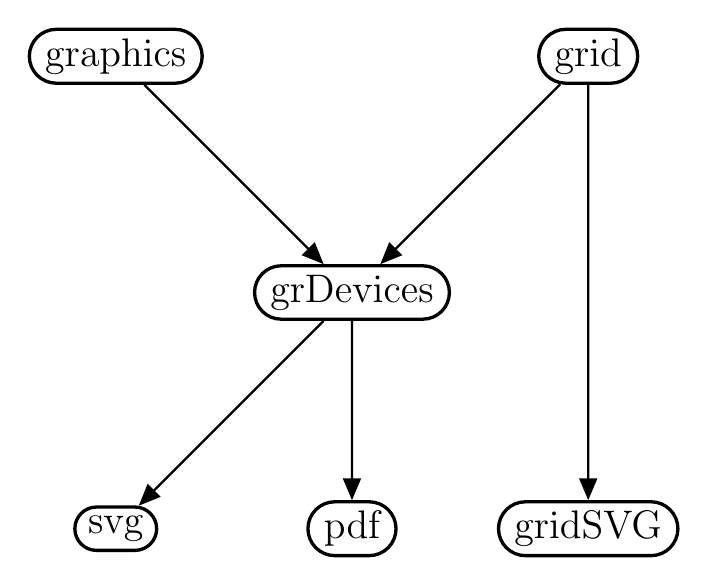
\begin{tikzpicture}[scale=3, >=triangle 45]
\tikzstyle{every node}=[draw,shape=circle];
\node[rounded rectangle, very thick] (grdev) at (1,1)  {\Large grDevices};
\node[rounded rectangle, very thick] (gr) at (0,2) {\Large graphics};
\node[rounded rectangle, very thick] (grid) at (2,2) {\Large grid};
\node[rounded rectangle, very thick] (svg) at (0,0) {\Large svg};
\node[rounded rectangle, very thick] (pdf) at (1,0) {\Large pdf};
\node[rounded rectangle, very thick] (gridsvg) at (2,0) {\Large gridSVG};
\draw [->, thick] (grdev) -- (svg);
\draw [->, thick] (grdev) -- (pdf);
\draw [->, thick] (gr) -- (grdev);
\draw [->, thick] (grid) -- (grdev);
\draw [->, thick] (grid) -- (gridsvg);
\end{tikzpicture}
\end{center}

\begin{minted}[frame=single]{r}
square <- function(x) {
  x * x
}
\end{minted}

\chapter{Conclusion}
\input{./tex/conclusion.tex}

%%%%%%%%%%%%%%%%%%%
% END MAIN MATTER %
%%%%%%%%%%%%%%%%%%%
 
\appendix
\input{./tex/appendix.tex}
 
%%%%%%%%%%%%%%%%%%%%
% BEGIN REFERENCES %
%%%%%%%%%%%%%%%%%%%%

\clearpage
\phantomsection
\addcontentsline{toc}{chapter}{References}
\input{./tex/references.tex}

\bibliographystyle{apa}
\bibliography{references.bib}

%%%%%%%%%%%%%%%%%%
% END REFERENCES %
%%%%%%%%%%%%%%%%%%

\end{document}
